\chapter{Marco Teórico}
 %\addcontentsline{toc}{chapter}{Marco Teórico}

\section{Minería de Datos}

La minería de datos (MD) es el proceso de encontrar patrones y relaciones en los datos con el fin de realizar actividades descriptivas y predictivas. La MD descriptiva busca descubrir en grandes volúmenes de datos las estructuras, relaciones, tendencias, grupos y valores atípicos que están contenidos en los datos. Por su parte, la MD predictiva construye modelos y procedimientos de regresión, clasificación, reconocimiento de patrones y tareas de aprendizaje de máquinas  que evalúan la capacidad predictiva de estos modelos en datos frescos o nuevos \cite{Izenman2006}. 
El modelamiento de los datos mediante las técnicas de MD puede ser usado para predecir el comportamiento de un individuo, segmentar una población, determinar las relaciones entre una población, determinar las características que más afectan a un resultado en particular; y en las empresas, estas técnicas tienen el objetivo de desarrollar estrategias para ser más competitivas en el mercado. Los datos de las compañías que se analizan pueden presentarse en todo tipo de formatos y estructuras y pueden estar almacenados en todo tipo de infraestructura \cite{Izenman2006}. Por esta razón la MD ha optado por clasificarse en varios tipos de funciones y técnicas que no se apartan del proceso tradicional para minar o extraer datos, como se ilustra en la Figura \ref{procesominar}.

\begin{figure}[h]
	\centering
	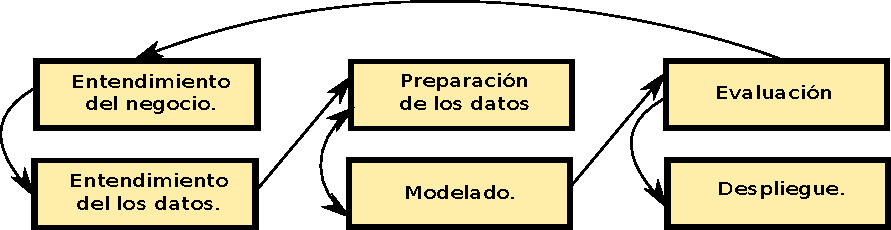
\includegraphics[width=\textwidth]{procesominar}
	\caption{Proceso Industrial estándar para minar datos.}
	\label{procesominar}
\end{figure}



La Figura \ref{procesominar}  ilustra el proceso empleado tradicionalmente en la MD, Cross Industry Standard Process for Data Mining  (CRISP-DM)\cite{Hornick2009}. Es importante diferenciar las técnicas o funciones que se aplican para cada una de las etapas de este proceso:
\begin{itemize}

\item{ \textbf{Entendimiento del negocio:}}
 El primer paso es el más importante, se llama entendimiento del negocio y se fundamenta en la identificación del problema, en esta fase se analiza qué recursos son pertinentes para solucionar el problema y en algunos casos el retorno de la inversión\cite{Hornick2009}.
\item{ \textbf{Entendimiento de los datos.}}
En este paso se deben identificar los datos a través de métodos estadísticos, por ejemplo, en qué rango de valores se encuentran los datos y qué fuentes de datos son necesarias para la solución del problema\cite{Hornick2009}.
\item{ \textbf{Preparación de los datos:}}
En esta etapa los datos ya se encuentran identificados y es necesario limpiarlos y formatearlos para presentarlos correctamente y no crear ambigüedad o manejar escalas de medición diferentes, por ejemplo, el género de los sujetos que aparece como masculino y femenino se muestra como 0 y 1 respectivamente\cite{Hornick2009}.
\item{ \textbf{Modelado:}}
En esta etapa es en donde se aplican las diferentes técnicas de regresión y clasificación para minar los datos dependiendo del análisis que el usuario haya realizado en la etapa de entendimiento del negocio\cite{Hornick2009}.
\item{ \textbf{Evaluación:}}
Esta etapa es necesaria para probar que el modelo alcanzó los objetivos y mostró los resultados esperados. Durante la etapa de evaluación se puede direccionar el esfuerzo a mirar aspectos que no se hayan cubierto en la etapa de modelado\cite{Hornick2009}.
\item{ \textbf{Despliegue:}}
La etapa de despliegue termina con un reporte. Una solución de minería de datos que se puede repetir y está integrada con el proceso de negocio de la compañía\cite{Hornick2009}.

\end{itemize}


Los datos históricos que se encuentran almacenados en los diferentes silos de datos en las compañías contienen una gran cantidad de registros que deben ser explorados para extraer el conocimiento. El descubrimiento de estos datos se conoce como conocimiento descubierto en bases de datos o KDD de sus siglas en inglés Knowledge discovery in databases\cite{Hornick2009}. Los procedimientos que se realizan para analizar estos datos se pueden clasificar en las siguientes técnicas y funciones:
\begin{itemize}
\item{ \textbf{Clasificación:}}
 Se usa para hacer predicciones en ejercicios como las encuestas, la segmentación de usuarios, el análisis de créditos bancarios, procesos estadísticos, detección de patrones, etc\cite{Izenman2006}. La clasificación de datos se realiza dependiendo de sus valores, por ejemplo, si se tiene a una persona que es de sexo femenino, y su estatura es mayor de 180 cm,  se clasifica su talla como L.
\item{ \textbf{Regresión:}}
Es usada para hacer predicciones en escenarios de datos continuos; es valiosa para el forecast, predicciones de series de tiempo y modelos médicos y ambientales\cite{Hornick2009}. La regresión a diferencia de la clasificación usa los datos de entrada para crear una función de entrenamiento y poder realizar pronósticos sobre estos datos de entrada\cite{Izenman2006}, por ejemplo, el valor de venta para una casa estará dado por la cantidad de baños multiplicado por su área.
\item{ \textbf{Atributo importancia:}}
En el análisis de negocio es muy importante identificar las características en los datos que influencian el comportamiento de los beneficios económicos\cite{Hornick2009}. Para tener una idea rápida de un dato como este, basta pensar en el estrato socioeconómico y su importancia para determinar el cobro de la cuenta de los servicios públicos.
\item{ \textbf{Asociación:}}
Es una técnica fuertemente usada en el análisis transaccional, se especializa en encontrar implicaciones en los datos o dependencias entre elementos repetidos en diferentes transacciones\cite{Hornick2009}.
\item{ \textbf{Clustering o Agrupamiento:}}
Esta es una función muy importante en la logística, en las cadenas de producción, en el análisis genético y en la minería de texto\cite{Hornick2009}. En el clustering se compara un objeto de un conjunto de datos contra muchos conjuntos de datos, el resultado de este algoritmo se llama dendrograma. Los algoritmos de clustering son iterativos y pueden retornar la distancia entre cada resultado o incluso crear jerarquías de los datos encontrados en los diferentes conjuntos o clúster. Los algoritmos más usados son: K-means clustering, K-medioids clustering, Hierarchical clustering, Kernel K-means, soft K-means, etc. La diferencia de los algoritmos radica en la función de distancia usada\cite{Izenman2006}.
\item{ \textbf{Predicción:}}
Es una función que ofrece una salida dependiendo de un conjunto histórico de datos; usa árboles de decisión y redes neuronales para argumentar su salida y procede dependiendo del conjunto de datos de entrada, por ejemplo puede ser usada para detectar defectos o calcular el mantenimiento de una máquina\cite{Hastie2009}.
\item{ \textbf{Estimación de densidad no paramétrica:}}
Es una técnica alternativa para el estudio de los datos multivariados, en donde estos datos no pertenecen a una distribución de probabilidad conocida. Como resultado al aplicar esta técnica se obtiene la estimación no paramétrica de una función de distribución de densidad para los datos\cite{Hornick2009}.
\item{ \textbf{Inferencia:}}
El objetivo de esta función consiste en estimar las relaciones existentes entre dos variables, especialmente como la variable dependiente cambia en función de las independientes, $Y=f(X)$. Se puede hablar de tres tipos de funciones en esta categoría, las funciones paramétricas, las funciones no paramétricas y las funciones semi paramétricas\cite{Izenman2006}.
\item{ \textbf{Remuestreo:}} 
El objetivo de estas técnicas es generar nuevos datos a partir de un modelo teniendo en cuenta la flexibilidad y el error. Las técnicas de remuestreo son muy costosas a nivel computacional y entre las funciones más usadas se encuentran Bootstrap y  Cross-Validation\cite{Elovici2003}.
\item{ \textbf{Subset selection:}}
Es una función de selección que identifica un grupo de predictores o asume unas variables $X$ que tiene mucha influencia en la variable respuesta $Y$, con esta información, la función crea un modelo que se ajusta a los predictores $X$ mediante la suma de sus cuadrados\cite{Hastie2009,Izenman2006}.
\item{ \textbf{Shrinkage or Regularization:}}
Es una función de selección de características que da muy buenos resultados por su ajuste a la varianza de los datos, estos métodos proponen seleccionar las variables que más aportan en la suma de cuadrados y penalizar las que no aportan [13]. Los algoritmos más conocidos que aplican esta función son Ridge Regression y Least Absolute Shrinkage and Selection Operation (LASSO) propuesto en 1996 por Tibshirani\cite{Hastie2009}. Las generalizaciones del algoritmo LASSO se han convertido en un tema de gran interés, entre las más importantes están: Generalized Linear Models (GLM), Elastic Net, Dantzig selector, SVN (Support Vector Machine), high dimensional matrix estimation y multivariate methods.
\end{itemize}

Es importartante considerar en esta sección que existe una relación entre las técnicas de la minería de datos y las funciones usadas en la minería de datos, cada técnica y función tiene su dominio y su contexto de uso, el cual varía según los tipos de datos y la finalidad en la implementación\cite{Harding2006}. \\
En búsqueda del propósito de construir modelos de características es necesario ampliar la información en los métodos que generen árboles y las soluciones a los problemas de agrupamiento, penalización y clasificación. Entre los más importantes están los árboles de regresión y clasificación (CART) y C4.5 y los bosques aleatorios de Leo Breiman. Los árboles de clasificación son métodos que tratan de dividir o partir los datos desde el principio hasta el final, estos métodos dedican su esfuerzo a estimar esos puntos de inicio y fin en los datos y la distancia de la partición o en número de tamaño de la división \cite{Izenman2006, Hastie2009}.
Un árbol es la representación de un conjunto de áreas, ahora bien, si los datos constituyen una nube de puntos, el árbol puede seleccionar las áreas en las cuales se divide dicha nube de puntos. Además de usar árboles, también es común implementar métodos predictivos como \textit{Bootstrap} o \textit{Cross validation} para ajustar los puntos a cada área y bajo este enfoque se desarrolla \textit{Random Forest} o árboles aleaorios\cite{Izenman2006, Hastie2009}.
La formación de las áreas a partir de un conjunto de datos está dada por los valores $X_{1}$ y $X_{2}$, se puede observar que la Ecuación \ref{eq1} representa los futuros puntos que se ubicarán en las $k$ regiones\cite{Izenman2006}. Esta es la representación de un árbol de regresión con $k$ regiones. Donde se estiman los valores de $f(X)$, los cuales están dados por los tamaños $c_{m}$ de las divisiones de los datos de entrada en el intervalo $(I)$ cuando estos pertenecen a una región $R_{m}$ determinada.

    \begin{equation}
    \hat{f}(X)=\sum_{\substack{m=1}}^kc_{m}I\{(X_{1},X_{2})\in R_{m}\}
    \label{eq1}
    \end{equation}

En la Ecuación \ref{eq1} se satisface la condición de asignación de los puntos a unas regiones señaladas como ramas de un árbol, donde la interpretabilidad puede verse reducida a medida de qué el árbol crezca o tenga más ramas. Un punto de discusión es la estimación del corte del árbol, esta decisión es delicada cuando se puede ver afectada por la variabilidad de las observaciones\cite{Izenman2006}, por ejemplo, la detección de spam en los correos electrónicos es un escenario en donde se usan estos modelos, aunque en este ejemplo la vida de una persona no se vea comprometida por la mala asignación de su correo, estos métodos también apoyan la selección de los pacientes que sufren de una enfermedad en el corazón\cite{Izenman2006}. Por otra parte, Las líneas de producto también tienen un modelo muy similar a la Ecuación \ref{eq1}, en la cual para definir familias de productos es necesario generar un árbol partiendo de la asignación de las características a las regiones que serán los segmentos del mercado.

\section{Ingeniería de Líneas de producto}

La ingeniería de líneas de producto (ILP) tiene como objetivo la producción de conjuntos de productos con más características comunes que diferentes, estas líneas de producto (LP) se han convertido en un paradigma viable para mejorar la productividad y la calidad de la producción en masa\cite{Benavides2010}. La producción en masa, es el legado de la revolución industrial y está definida como la producción de un conjunto estandarizado de un mismo producto, en donde la personalización de este se convierte en un reto interesante para las compañías de cualquier tipo, inclusive para las empresas de desarrollo de software. Las características en los productos son el insumo en la LP, su razón de ser. Un producto tiene diversas características que pueden representarse en un modelo de características, por esta razón los modelos de características son comúnmente la representación de las LP \cite{Simpson, Zhang2013,Zhou2015b}.\\

Las LP protagonizan la etapa de diseño de los nuevos productos que consumen los clientes y la MD se especializa en extraer la información sobre la tendencia de los clientes en el mercado, la integración de estas dos tecnologías proporciona a las empresas información útil para el desarrollo de nuevos productos que se adapten a las necesidades de la sociedad\cite{Bae2011,Lin2013}. La MD puede solucionar una gran cantidad de problemas relacionados con el entendimiento de datos científicos (¿Cuáles son las causas raíces de un error?) y datos de negocios de cualquier dominio (¿Cuál es el producto que compran más sus clientes?)\cite{Hornick2009,Bae2011}. Saber qué se puede producir, con la certeza de ser comprado es lo que motiva a las compañías a crear productos de manera masiva y mejorar su producción para hacerla cada vez más rápida y flexible\cite{Benavides2010}. Estas tecnologías aplican para cualquier tipo de dominio y es de vital importancia para la salud del planeta reciclar estos datos, porque las empresas al saber la demanda de sus productos y servicios pueden afinar sus procesos de producción, ahorrando dinero y recursos\cite{Lian2015}. Estos productos pueden ser software también, incorporar LP en el ciclo de vida de desarrollo de software (CVDS) mejora las estadísticas de mercadeo ampliando los beneficios de dos a siete veces\cite{Zhang2013}.

\section{Modelos de características}

Un modelo de características (MC) representa la información de todos los posibles productos en una LP en términos de las características y las relaciones entre ellas \cite{Zhou2013}. En la Figura \ref{featuremodelgato} se elaboro un ejmplo sencillo para mostrar la representación de las caracteristicas de un gato sin embargo recomendamos a diferentes autores y sus representaciones\cite{Santos2015, Felfernig2015, TerBeek2015, Al2013}.
\begin{figure}[h]
	\centering
	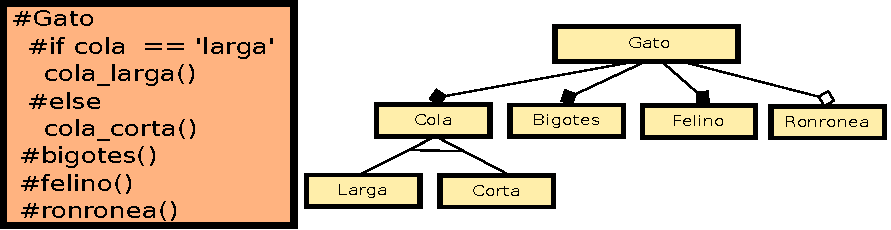
\includegraphics[width=\textwidth]{featuremodelgato}
	\caption{Modelo de caracteristicas de ejemplo representando un gato.}
	\label{featuremodelgato}
\end{figure}

En la literatura anterior se agrupan las características y sus relaciones de forma jerárquica, las relaciones pueden ser Obligatorio, Opcional, Alternativo, O, inclusión y exclusión\cite{Benavides2010}.
\begin{itemize}
\item{ \textbf{Obligatoria:}}
Esto significa que el hijo asignado tiene que estar incluido en el producto.
\item{ \textbf{Opcional:}}
Esto significa que el hijo asignado puede o no tener esta característica.
\item{ \textbf{Alternativo:}}
Da a conocer que solo una característica en la jerarquía puede ser seleccionada.
\item{ \textbf{O:}}
Esta relación significa que se puede seleccionar todas o ninguna de las características en la jerarquía.
Requerida: Cuando una característica requiere a otra, esta no puede existir sin la presencia de la otra.
\item{ \textbf{Exclusión:}}
Si una característica excluye a otra da a entender que las características seleccionadas no pueden ser parte del mismo producto.
\end{itemize}


La comunidad ha creado herramientas de ingeniería de software asistido por computadora, \textit{Computer Aided Software Engineering (CASE)} para el modelamiento y la configuración de los modelos de características, aunque están en constante desarrollo, se conocen algunas muy populares comoRECoVar\cite{Zhang2013,Bezerra2016}, VariaMos\cite{Mazo2015}, la cual tiene como objetivo desarrollar  familias de sistemas y también tiene herramientas para realizar operaciones sobre otros modelos. SPLOT (software product line online tool)\cite{Mendonca:2009:SSP:1639950.1640002}, la cual es una herramienta online para la configuración de características y la derivación de productos a partir de diagramas de características y modelos de variabilidad. La intención de esta investigación no será competir con estas herramientas sino complementarlas y extender su funcionalidad a la adquisición de datos que ofrecen las técnicas de agrupamiento dentro de la minería de datos.

	
